\documentclass[10pt,conference]{IEEEtran}

\usepackage{cite}
\usepackage{amsmath,amssymb,amsfonts}
\usepackage{algorithmic}
\usepackage{graphicx}
\usepackage{textcomp}
\usepackage{xcolor}
\usepackage{booktabs}
\usepackage{longtable}
\usepackage{array}
\usepackage{multirow}
\usepackage{wrapfig}
\usepackage{float}
\usepackage{colortbl}
\usepackage{pdflscape}
\usepackage{tabu}
\usepackage{threeparttable}
\usepackage{threeparttablex}
\usepackage[normalem]{ulem}
\usepackage{makecell}

\def\BibTeX{{\rm B\kern-.05em{\sc i\kern-.025em b}\kern-.08em
    T\kern-.1667em\lower.7ex\hbox{E}\kern-.125emX}}

\begin{document}

\title{Convolutional Neural Networks for the Prediction of ASD and 
       Biomarker Identification}

\author{
    \IEEEauthorblockN{Tony Kabilan Okeke}
    \IEEEauthorblockA{\textit{School of Biomedical Engineering} \\
    \textit{Drexel University}\\
    Philadelphia, PA \\
    tko35@drexel.edu}
}

\maketitle

% \begin{abstract}
%     The abstract will go here.
% \end{abstract}

% \begin{IEEEkeywords}
%     connectomics, CNN, biomarker, autism, ASD
% \end{IEEEkeywords}

% ----------------------------------------------------------------------------------------

\section{Introduction}

Autism Spectrum Disorder (ASD) is a neurodevelopmental disorder that is characterized by 
social and communicationdeficits as well as restricted, repetitive behaviors. Early 
diagnosis and intervention are critical for improvinglong-term outcomes; however, the 
current gold standard assessment tools are limited in their ability to accurately and 
efficiently diagnose ASD, particularly in young children. Typically, ASD diagnoses are 
based on behavioral criteria, but there is growing interest in the identification of 
objective biomarkers to aid in the diagnoses \cite{Shen.2019}. Biomarkers are measurable 
characteristics that can be used to indicate the presence or severity of a disease. In the 
case of ASD, biomarkers could be used to improve and validate diagnoses, especially in 
young children, and potentially before the emergence of symptoms.

Due to advancements in multimodal neuroimaging in recent years, neuroscience has gained 
unprecedented opportunities to interrogate the living human brain at multiple scales in 
both health and disease \cite{Hong.2019}, and these advancements have been especially 
useful in the study of neurodevelopmental disorders \cite{Nunes.2019}. The field of 
network neuroscience aims to investigate such disorders by leveraging magnetic resonance 
imaging (MRI) and and various tractography algorithms to construct `brain graphs' or 
`connectomes' which are matrix representations of the structural and/or functional 
connections between various regions of the brain. 

Several studies have been conducted to examine changes in functional connectivity in 
individuals with ASD relative to typically developing controls \cite{Lau.2019, Williams.2013}. 
However, less is known about changes in structural connectivity in individuals with ASD. 
By capitalizing on diffusion-weighted magnetic resonance imaging (dMRI), previous studies 
were able to identify abnormalities in the connectivity strength of several inter-regional 
fiber pathways in individuals with ASD \cite{dAlBbis.2018}. Despite the identification of 
these abnormalities, the diagnosis of ASD based on brain imaging remains a challenge. 
One reason for this challenge is that the abnormalities associated with ASD are often 
subtle and are often difficult to detect. This calls for the application of sophisticated 
computational methods to aid in the diagnoses.

In recent years, there has been an explosion of interest in the potential of machine 
learning to revolutionize different aspects of neuroscience \cite{Abos.2017,Vogt.2018}. 
However, given the complex and high-dimensional nature of connectomes, traditional 
machine learning approaches are not well-suited for connectome classification problems. 
Recent advances in deep learning, specifically Convolutional Neural Networks (CNNs), have 
shown promise in the prediction of clinical neurodevelopmental outcomes from brain 
networks (connectomes). For example, \textit{BrainNetCNN} was developed for the 
prediction of cognitive and motor scores from the connectomes of infants born preterm 
\cite{Kawahara.2017}.

In this study, we propose a novel convolutional neural network (CNN) architecture capable 
of distinguishing between connectomes of autistic and typically developing children. We 
will also attempt to identify biomarkers that better identify ASD in children. We will 
utilize graph theory measures as the features for our model. Additionally, we will
analyze the relationships between the potential biomarker(s) and autism severity, social
communication, and intellegence as assessed by the Autism Diagnostic Observation Schedule
Clinical Severity Score (ADOS-CSS), Social Communication Questionaire (SCQ) score, and
Intelligence Quotient (IQ) respectively.

% ----------------------------------------------------------------------------------------

\section{Materials and Methods}

Fig. \ref{project-schematic} provides an overview of the proposed approach for the 
development of a CNN-based classifier for ASD. In this section, we first describe the 
dataset used and the methodology involved in the generation of the structural connectomes 
from the raw MRI image data. We then describe the calculation of graph-therory measures
which will serve as features for the classifier. We also describe the exploratory analysis 
performed as well as the application of various feature selection techniques in an attempt
to identify potential biomarkers for ASD and reduce the feature space for the classifier.

\begin{figure*}[ht]
    \vskip 0.2in
    \begin{center}
        \centerline{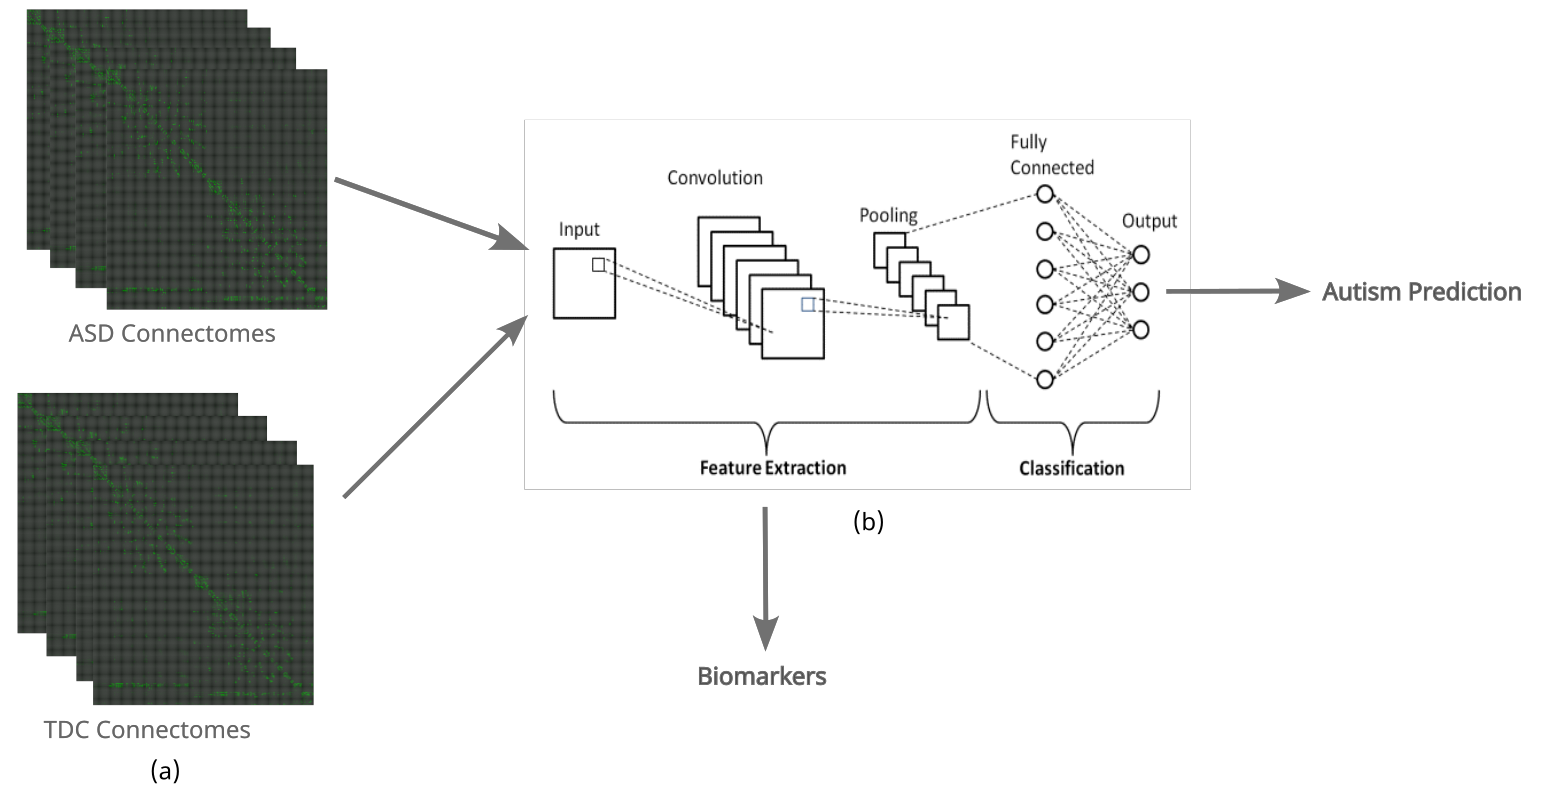
\includegraphics[width=6in]{../img/project_schematic_v1.png}}
        \caption{
            Overview of autism prediction and biomarker identification using a 
            Convolutional Neural Network based classifier. (a) (top) Structural 
            connectomes of patients with Autism Spectrum Disorder. (bottom) Structural 
            connectomes of Typically Developing Controls. (b) Schematic diagram for 
            convolutional neural network.
        }
        \label{project-schematic}
    \end{center}
    \vskip -0.2in
\end{figure*}

\textit{Dataset.} This study was conducted data provided by our collaborators at Penn 
Medicine. dMRI scans were collected from a cohort of 313 children between 6 and 19 years
old, including children with ASD ($n=163$; $\text{age}=12.10~\pm~2.76$; 133 males; 30 females) 
as  well as typically developing controls ($n=160$; $\text{age}=11.87~\pm~2.82$; 115 males; 35 females). 
For each subject, only a single dMRI scan was performed. The age, sex, Social 
Communication Questionnaire (SCQ) score, and IQ were recorded for all subjects in the 
cohort. The SCQ score is considered the gold standard measure of communication skills,
and ranges from 0 to 39; a score of 15 or higher is considered to be indicative of ASD, 
whereas a score of 14 or below is within the range of typical development. For subjects 
with ASD, the Autism Diagnostic Observation Schedule Calibrated Severity Score (ADOS-CSS) 
was also recorded. The ADOS Clinical Severity Score is a semi-structured, play-based 
assessment administered by a trained professional; iit is the gold-standard measure for 
autism severity and ranges from 1 to 10, with higher scores indicating greater severity 
of autism.

\textit{Connectomes.} Two connectomes were obtained from each dMRI scan; the first set 
of structural connectomes were construced using the Desikan atlas to define nodes, 
while the second set of connectomes were constructed using nodes defined by the 
Schaefer atlas. The Desikan atals parcellates the brain into 86 distinct regions while 
the Schaefer atlas parcellates the brain into 220 regions. The adjacency matrices for 
the Desikan connectomes were 86 x 86 in size. Whereas, the adjacency matrices for the
Schaefer connectomes were 220 x 220 in size. The edges for both sets of connectomes
were generated using tractographic tools.

\textit{Graph Theory Measures.} Several graph theory measures were computed for each set
of connectomes. The `bctpy' package -- a python-based implementation of the Brain 
Connectivity Toolbox -- was used to compute graph theory measures \cite{Rubinov.2010.BCT}. 
Both node-level and network-level measures were computed and compared using the 
two-sample t-test with variances assumed to be unequal; the Cohen's d effect sizes were 
also calculated for each comparison. 
% and the p-values were corrected for multiple comparisons using the Bonferroni method.

\textit{Exploratory Analysis.} In order to identify potential biomarkers from the computed 
graph theory measures, an exploratory analysis was performed. The association between 
the graph theory measures and autism severity was assessed by fitting the data to 
linear fixed-effects models to account for the effects of any covariates. The exploratory
analysis was performed in the R \cite{R-Core} and figures were generated using the 
`ggplot2' and `ggstatsplot' packages \cite{ggplot2, ggstatsplot}.

\textit{Biomarker Discovery.} Multiple feature selection techniques were evaluated in an 
attempt to identify potential biomarkers from the graph theory measures. The 
`scikit-learn' package was used to perform feature selection in python \cite{sklearn}. 
Univariate feature selection was performed using the `SelectKBest' function, and 
statistical significance was assessed using the ANOVA F-scores for each measure. 
Additionally, the data were fit to machine learning classification models (including
Support Vectorm Machine and Random Forest) to distiguish between ASD and TDC connectomes. 
Recursive feature elimination was then used to identify potential biomarkers based on
the important features in each model.

% ----------------------------------------------------------------------------------------

\section{Results}

    \subsection{Comparison of Global Graph Theory Measures.} 
    In order to reduce the number of features in the dataset, calculated the group 
    difference between ASD and TDC for each of the computed global graph theory measures.
    Fig. \ref{group-diff-boxplot-global-measures} shows boxplots comparing six global graph
    theory measures for ASD and TDC. Measures with p-values below 0.05 were identified and
    included when training machine learning models. Of the 37 global graph theory measures
    calculated, the following were found to be significant: Average degree, 
    degree between modules, degree within modules, inter-hemispheric degree, density and 
    eigenvector centrality. The Cohen's d effect sizes and p-values for each of the 6 
    global graph theory measures are shown in Table \ref{group-diff-global-measures}.

    \begin{figure}[ht]
        \vskip 0.2in
        \begin{center}
            \centerline{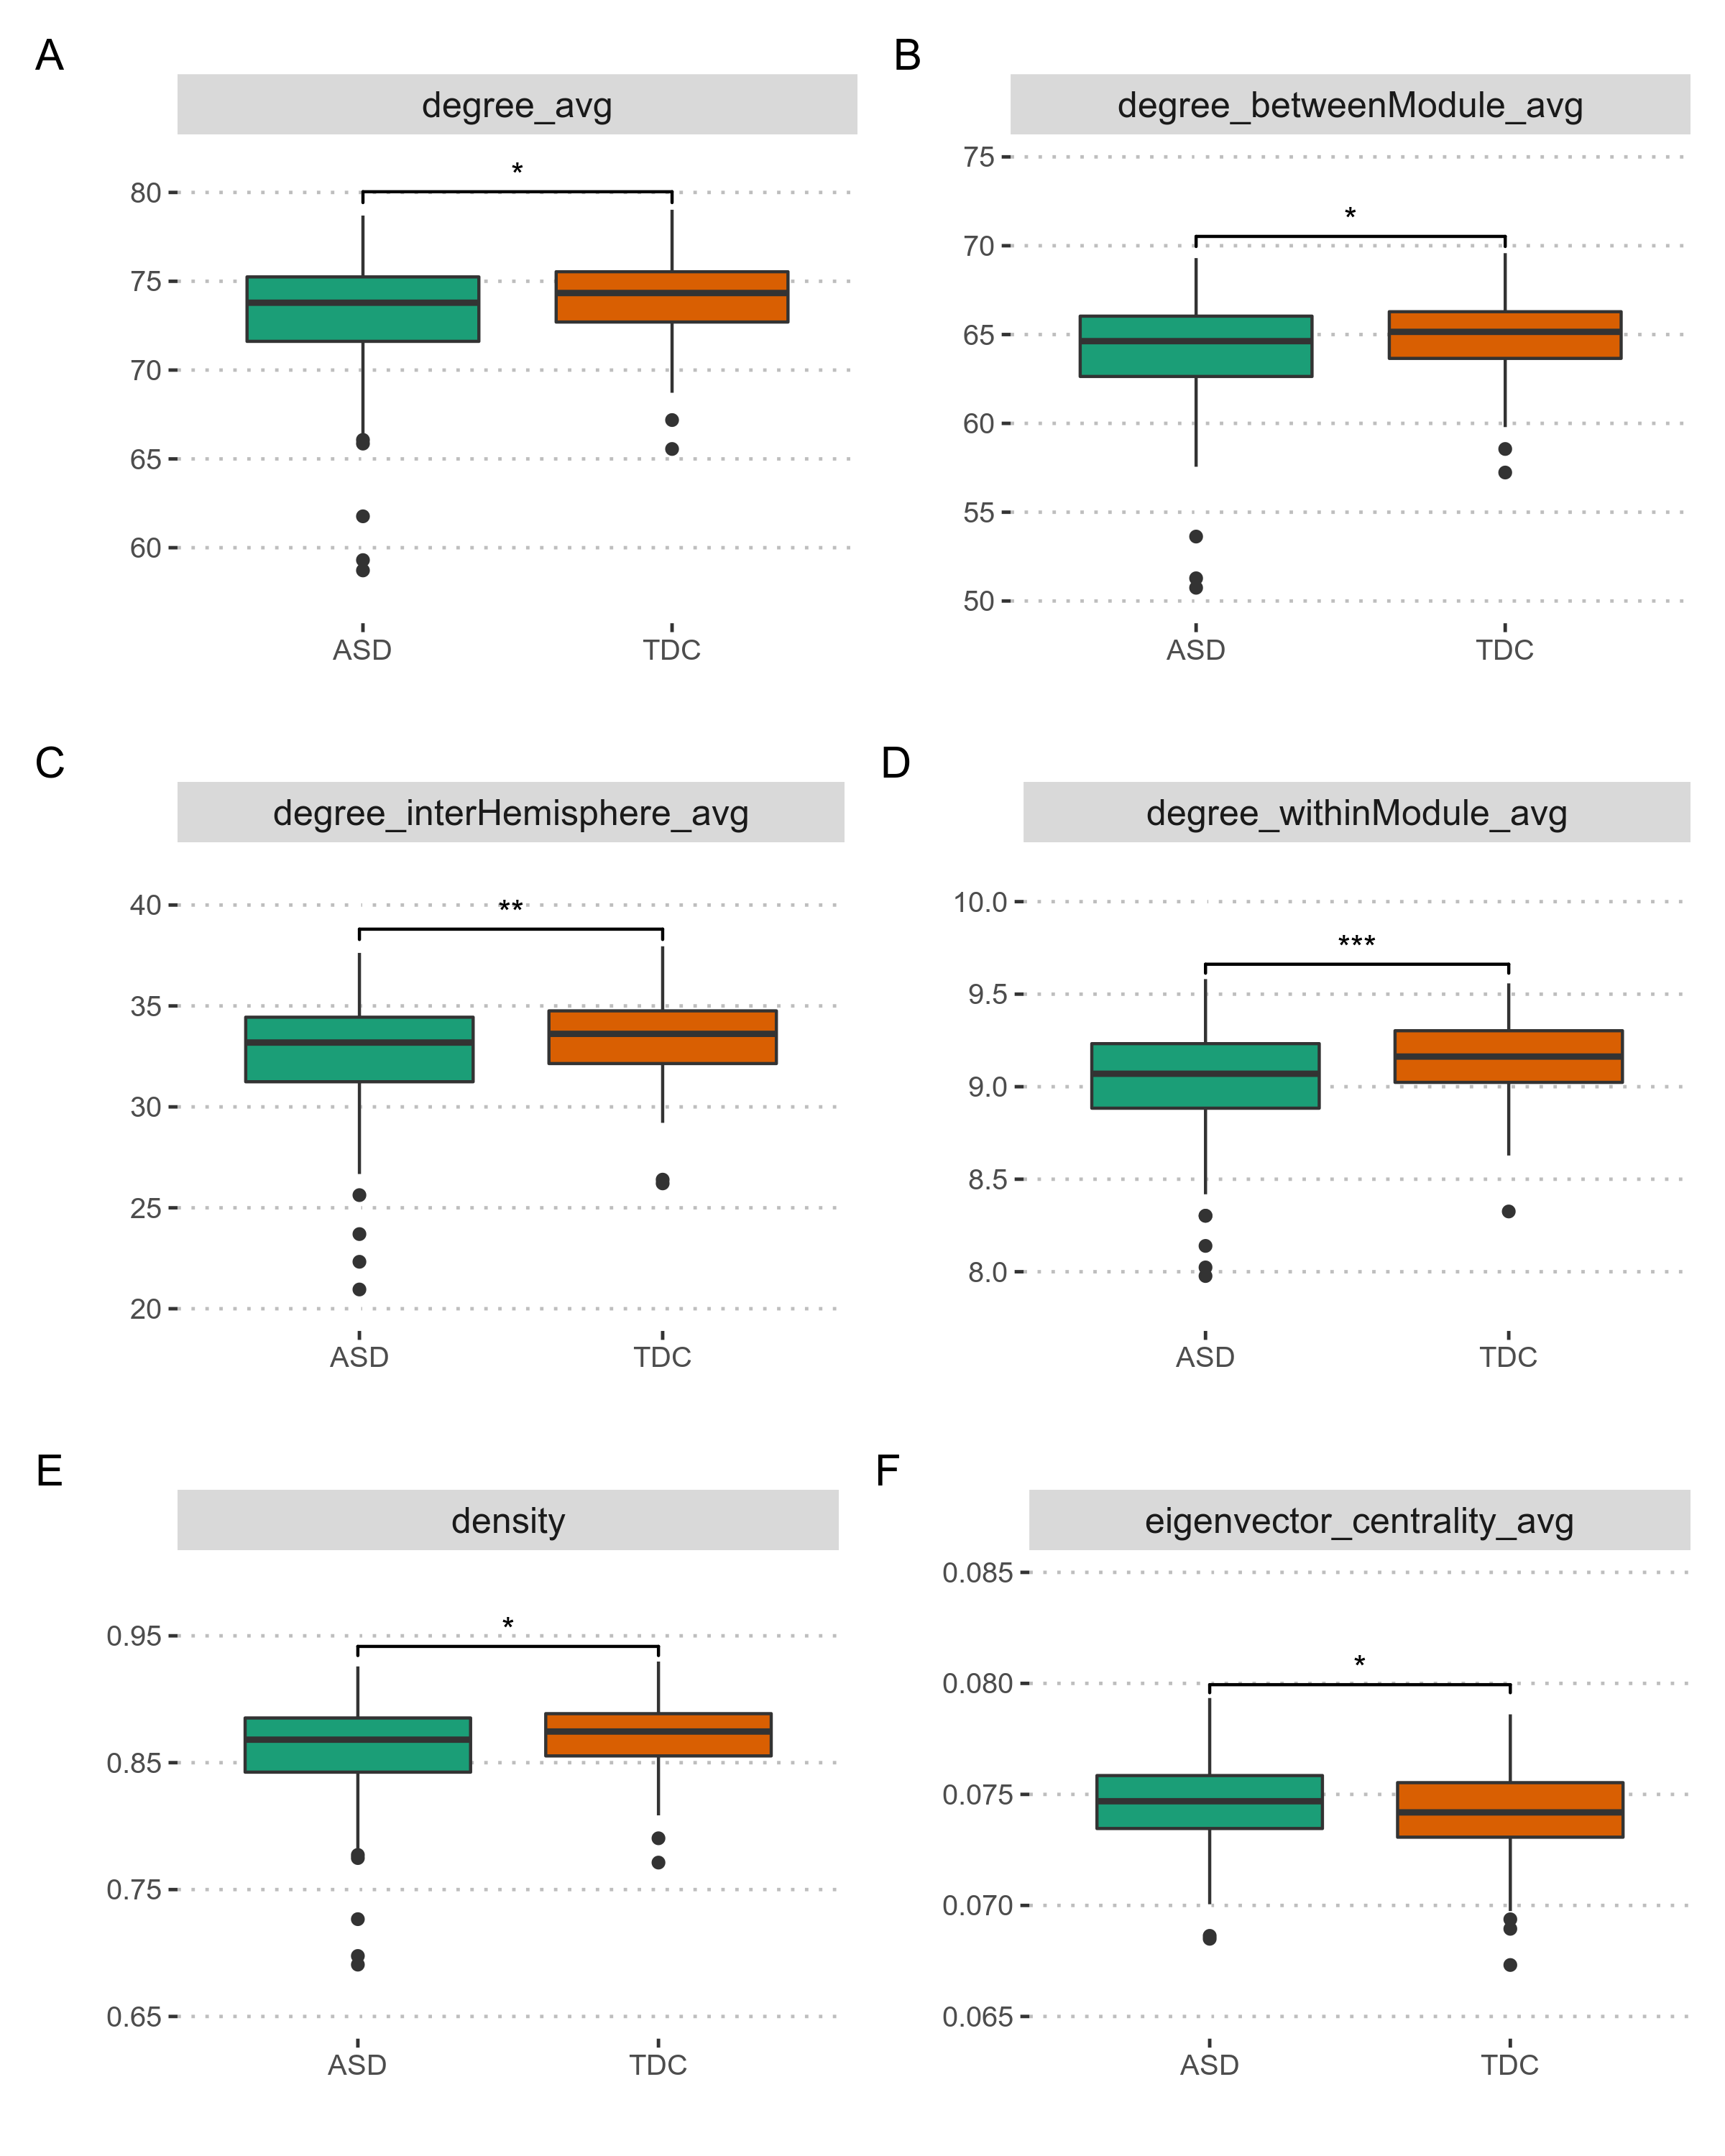
\includegraphics[width=\columnwidth]{../../AutismCNN/figures/group-diff_global-measures_boxplot.png}}
            \caption{
                Significant Group differences between ASD and TDC connectomes for six graph
                theory measures. The significance is indicated by the starts `*' above the
                braces in each sub-plot. (A) Average Degree (B) Average Degree Between Modules
                (C) Average Inter-Hemispheric Degree (D) Average Degree Within Modules
                (E) Network Density (F) Average Eigenvector Centrality
            }
            \label{group-diff-boxplot-global-measures}
        \end{center}
        \vskip -0.2in
    \end{figure}

    \begin{table}
        \caption{Group differences between ASD and TDC for Global Graph Theory Measures.}
        \begin{center}
            \begin{tabular}{lrr}
                \toprule
                Measure & p & Cohens\_d\\
                \midrule
                Average Degree Within Module & 1.89e-05 & -0.4886968\\
                Average InterHemispheric Degree & 5.46e-03 & -0.3147607\\
                Average Degree & 1.05e-02 & -0.2891104\\
                Density & 1.05e-02 & -0.2891106\\
                Average Degree Between Modules & 1.83e-02 & -0.2665902\\
                Average Eigenvector Centrality & 4.98e-02 & 0.2225106\\
                \bottomrule
            \end{tabular}
            \label{group-diff-global-measures}
        \end{center}
    \end{table}

    The global graph theory measures were then correlated with IQ, ADOS-CS, and SCQ scores.
    No significant correlations were observed between with SCR or ADOS-CS scores. The
    average inter-hemispheric degree and average degree within modules were found to 
    exhibit significant, weak correlations with IQ scores among autistic children.
    Fig. \ref{corrplot-global-measures} shows linear regression lines fitted to the data;
    the scatter plots are annotated with the correlation coefficient (R) and p-value for
    each case.

    \begin{figure}[ht]
        \vskip 0.2in
        \begin{center}
            \centerline{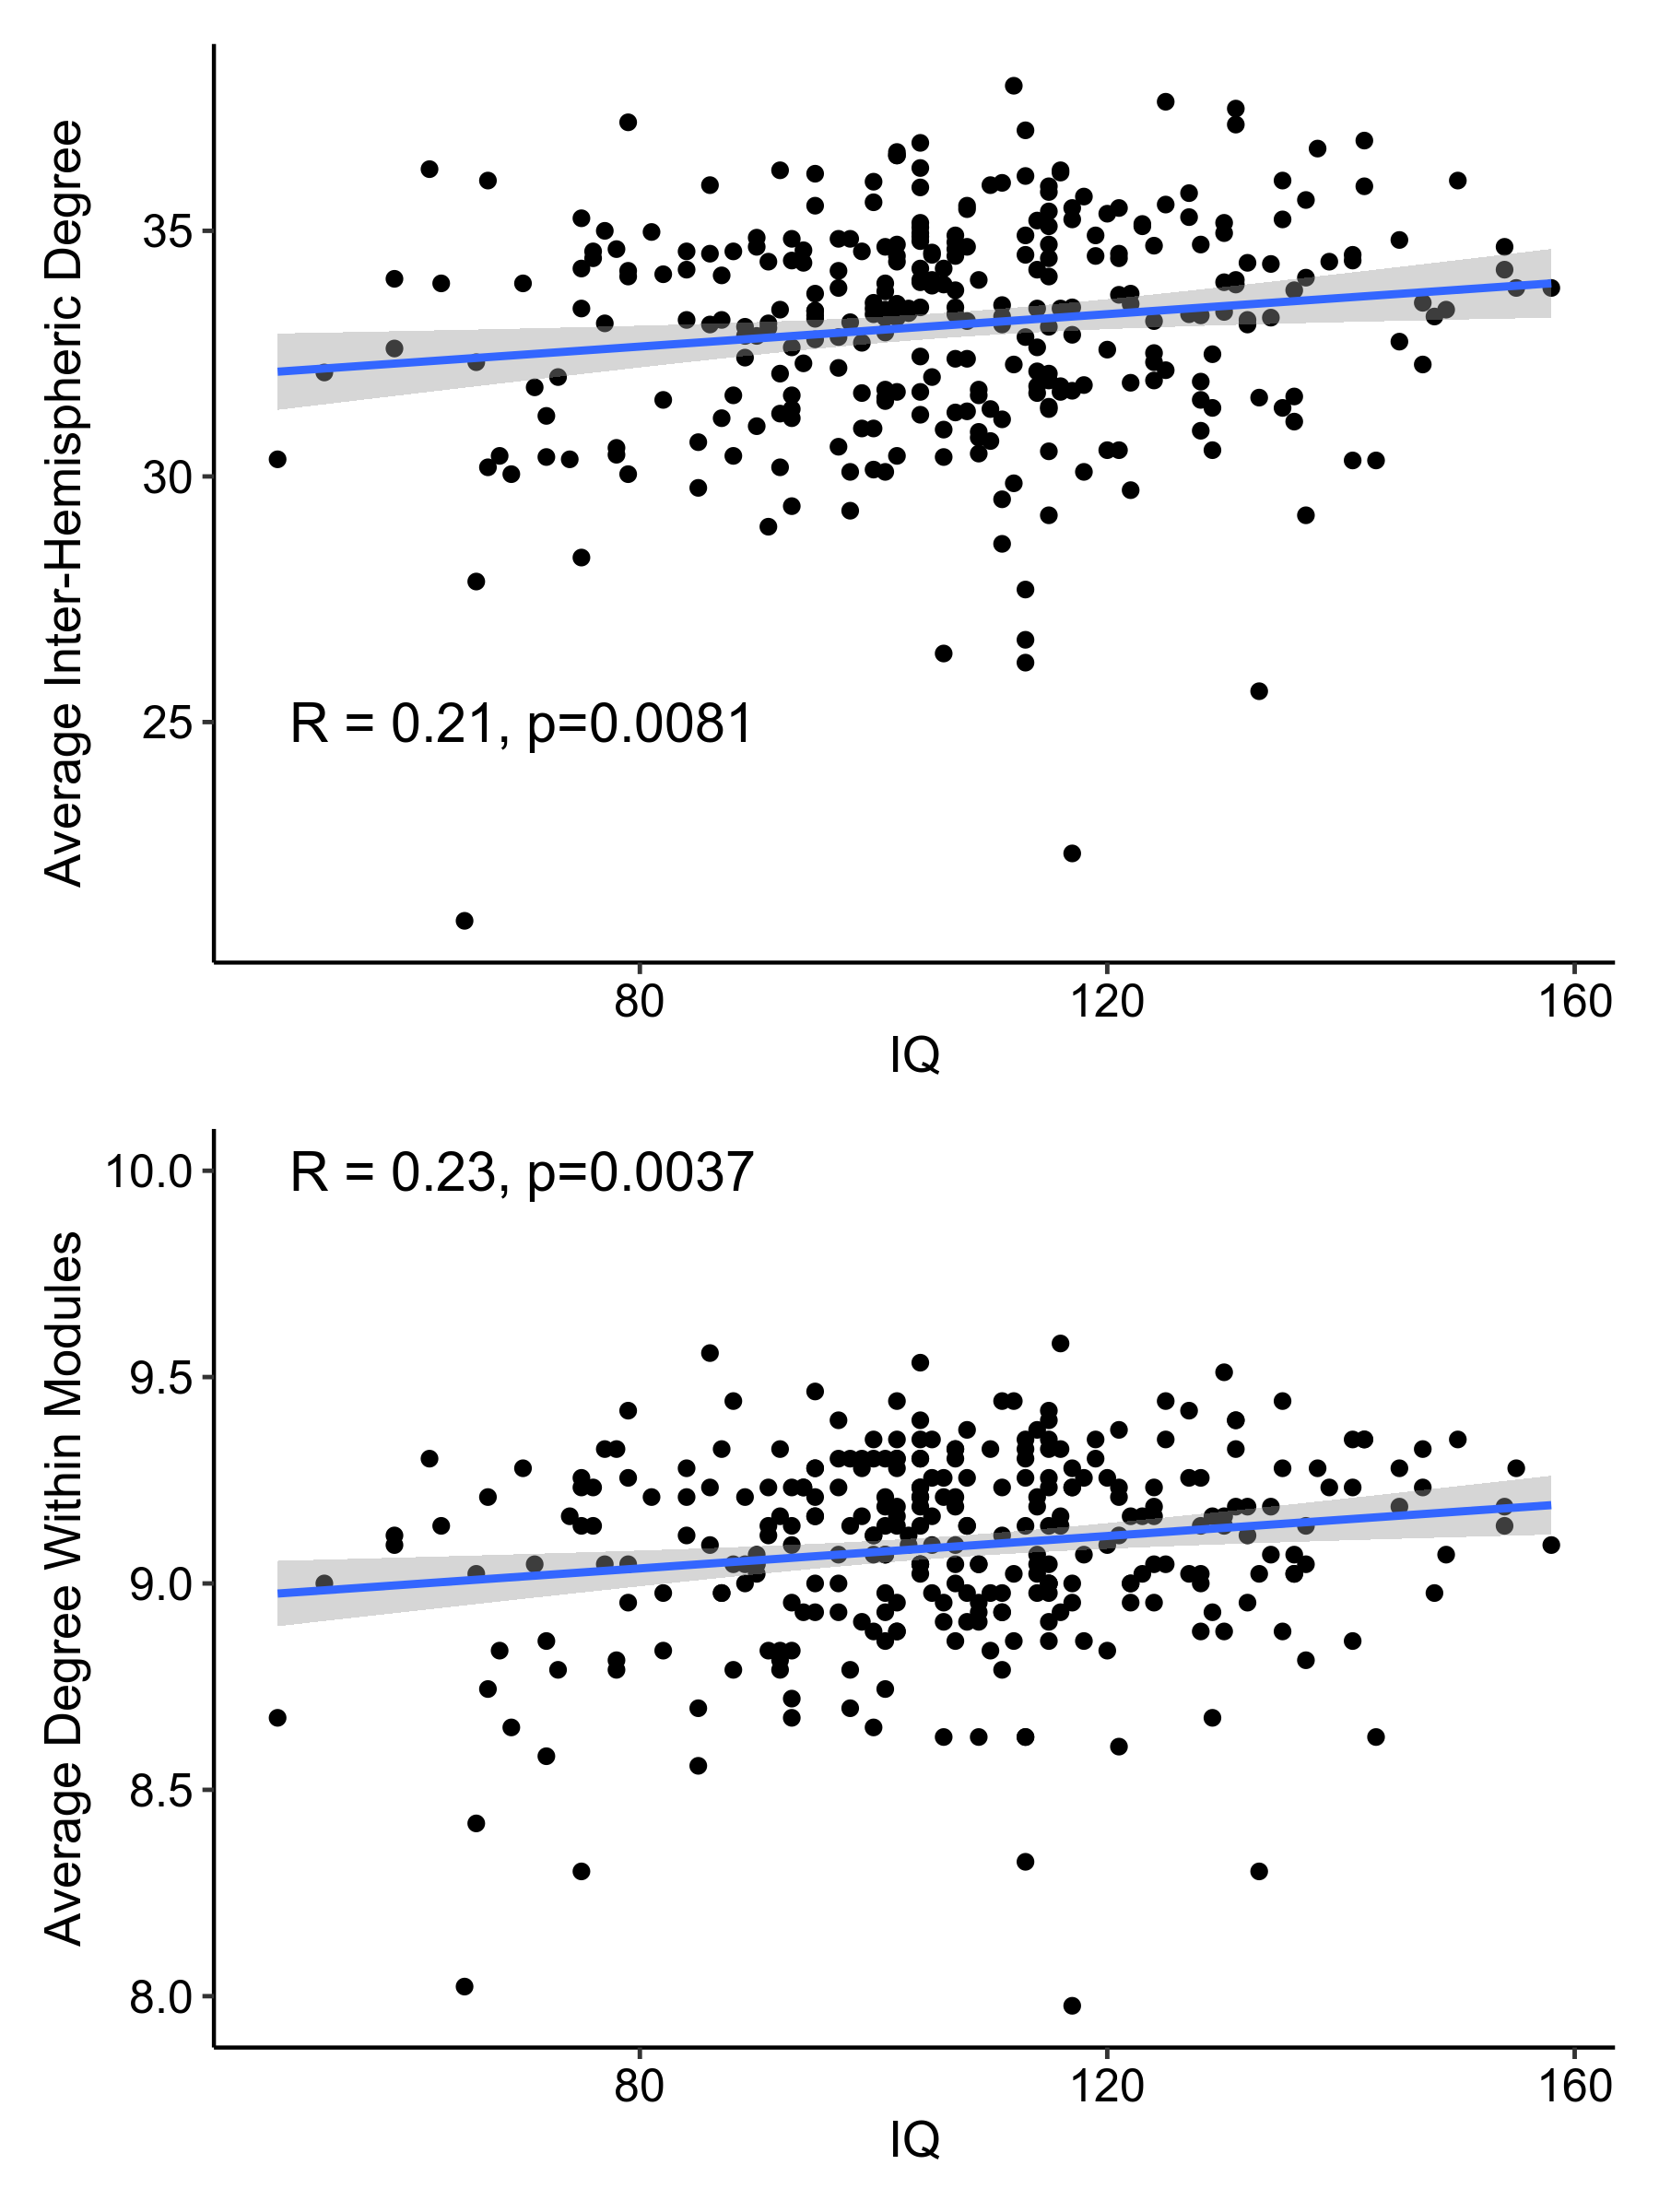
\includegraphics[width=\columnwidth]{../../AutismCNN/figures/corrplot_global-measures_boxplot.png}}
            \caption{
                Scatterplots with fitted linear regression lines for global graph theory 
                measures significantly correlated with IQ. (Top) Average Inter-Hemispheric 
                Degree  (Bottom) Average Degree Within Modules
            }
            \label{corrplot-global-measures}
        \end{center}
        \vskip -0.2in
    \end{figure}


% ----------------------------------------------------------------------------------------

\newpage

\begin{thebibliography}{00}
    \bibitem{Abos.2017} {Abos, A., Baggio, H., Segura, B., Garcia-Diaz, A., Compta, Y., Marti, M., Valldeoriola, F., \& Junqué, C. (2017). Discriminating cognitive status in Parkinson’s disease through functional connectomics and machine learning. Scientific reports, 7(1), 1–-13.}
    \bibitem{dAlBbis.2018} {d`Albis, M.A., Guevara, P., Guevara, M., Laidi, C., Boisgontier, J., Sarrazin, S., Duclap, D., Delorme, R., Bolognani, F., Czech, C., \& others (2018). Local structural connectivity is associated with social cognition in autism spectrum disorder. Brain, 141(12), 3472–-3481.}
    \bibitem{Craddock.2013} {Craddock, R., Jbabdi, S., Yan, C.G., Vogelstein, J., Castellanos, F., Di Martino, A., Kelly, C., Heberlein, K., Colcombe, S., \& Milham, M. (2013). Imaging human connectomes at the macroscale. Nature methods, 10(6), 524–-539.}
    \bibitem{Hong.2019} {Hong, S.J., Wael, R., Bethlehem, R., Lariviere, S., Paquola, C., Valk, S., Milham, M., Di Martino, A., Margulies, D., Smallwood, J., \& others (2019). Atypical functional connectome hierarchy in autism. Nature communications, 10(1), 1–-13.}
    \bibitem{Kawahara.2017} {Kawahara, J., Brown, C., Miller, S., Booth, B., Chau, V., Grunau, R., Zwicker, J., \& Hamarneh, G. (2017). BrainNetCNN: Convolutional neural networks for brain networks; towards predicting neurodevelopment. NeuroImage, 146, 1038-–1049.}
    \bibitem{Lau.2019} {Lau, W., Leung, M.K., \& Lau, B. (2019). Resting-state abnormalities in autism spectrum disorders: a meta-analysis. Scientific reports, 9(1), 1–-8.}
    \bibitem{Nunes.2019} {Nunes, A., Peatfield, N., Vakorin, V., \& Doesburg, S. (2019). Idiosyncratic organization of cortical networks in autism spectrum disorder. Neuroimage, 190, 182-–190.}
    \bibitem{Osmanlioglu.2019} {Osmanlioglu, Y., Tunc, B., Parker, D., Elliott, M., Baum, G., Ciric, R., Satterthwaite, T., Gur, R., Gur, R., \& Verma, R. (2019). System-level matching of structural and functional connectomes in the human brain. NeuroImage, 199, 93–-104.}
    \bibitem{sklearn} {Pedregosa, F., Varoquaux, G., Gramfort, A., Michel, V., Thirion, B., Grisel, O., Blondel, M., Prettenhofer, P., Weiss, R. et. al. (2011). Scikit-learn: Machine Learning in Python. Journal of Machine Learning Research, 12(1), 2825-2830.}
    \bibitem{ggstatsplot} {Patil, I. (2021). Visualizations with statistical details: The `ggstatsplot' approach. Journal of Open Source Software, 6(61), 3167, doi:10.21105/joss.03167.}
    \bibitem{R-Core} {R Core Team (2022). R: A language and environment for statistical computing. R Foundation for Statistical Computing, Vienna, Austria. URL https://www.R-project.org/.}
    \bibitem{Rubinov.2010.BCT} {Rubinov, M., \& Sporns, O. (2010). Complex network measures of brain connectivity: uses and interpretations. Neuroimage, 52(3), 1059-–1069.}
    \bibitem{Salari.2020} {Sherkatghanad, Z., Akhondzadeh, M., Salari, S., Zomorodi-Moghadam, M., Abdar, M., Acharya, U., Khosrowabadi, R., \& Salari, V. (2020). Automated detection of autism spectrum disorder using a convolutional neural network. Frontiers in neuroscience, 13, 1325.}
    \bibitem{Shen.2019} {Shen, L., Zhao, Y., Zhang, H., Feng, C., Gao, Y., Zhao, D., Xia, S., Hong, Q., Iqbal, J., Liu, X., \& others (2019). Advances in biomarker studies in autism spectrum disorders. Reviews on Biomarker Studies in Psychiatric and Neurodegenerative Disorders, 207–-233.}
    \bibitem{Tunc.2021} {Tunç, B., Pandey, J., St. John, T., Meera, S., Maldarelli, J., Zwaigenbaum, L., Hazlett, H., Dager, S., Botteron, K., Girault, J., \& others (2021). Diagnostic shifts in autism spectrum disorder can be linked to the fuzzy nature of the diagnostic boundary: a data-driven approach. Journal of Child Psychology and Psychiatry, 62(10), 1236–-1245.}
    \bibitem{Vogt.2018} {Vogt, N. (2018). Machine learning in neuroscience. Nature Methods, 15(1), 33–-33.}    
    \bibitem{ggplot2} {Wickham, H., ggplot2: Elegant Graphics for Data Analysis. Springer-Verlag New York, 2016.}
    \bibitem{Williams.2013} {Williams, D., Cherkassky, V., Mason, R., Keller, T., Minshew, N., \& Just, M. (2013). Brain function differences in language processing in children and adults with autism. Autism Research, 6(4), 288–-302.}

\end{thebibliography}

\end{document}
